\documentclass[a4paper, 10pt]{ctexart} %中文支持
\usepackage{float}              %防止浮动元素浮动
\usepackage{rotating}           %旋转图片
\usepackage{amsfonts}           %对某一些字体之支持
\usepackage{mathrsfs}           %mathscr e.g.
\usepackage[]{amsmath}          %数学公式
\usepackage{amsthm}             %定义, 定理, 证明, 例子环境的支持
%使用方法:
%\newtheorem{environment name}{caption}
%比如 \newtheorem{example}{这是例子}
%效果 \begin{example} xxx \end{example} -> 这是例子 1 xxx
%proof就不需要了
\usepackage{graphicx}           %插入图片
\usepackage[left=1.25in,right=1.25in,top=1in,bottom=1in]{geometry}   %用来排版的
\usepackage{color}            %给部分文本上色的
\usepackage{algorithm}          %写伪代码的
%\usepackage{algorithmic}       %同上
\usepackage{algorithmicx}
\usepackage{algpseudocode}
\usepackage{minted}
\usepackage{amssymb}            %用来加入一些数学符号, 比如说 $\varnothing$
\usepackage{titlesec}
\usepackage{fontspec}           %不知道用来干嘛的
\usepackage{hyperref}           %生成可跳转的书签
% -------------------------------
\setmonofont{Ubuntu Mono}       %?
\usemintedstyle{custommanni}    %设置minted插入代码的风格
\titleformat*{\section}{\huge\bfseries}             %管理title的字体和大小
\titleformat*{\subsection}{\Large\bfseries}         %bfseries就是默认的字体.
\titleformat*{\subsubsection}{\large\bfseries}
% -------------------------------
\newtheorem{theorem}{Theorem}
\newtheorem{example}{Example}
\newtheorem{definition}{Definition}
\newtheorem{lemma}{Lemma}
\newtheorem{remark}{Remark}
\newtheorem{corollary}{Comment}
\newtheorem{proposition}{Proposition}
\pagestyle{plain}
\title{chapter 6: search strategy}
\author{You \and Me}
\date{date: Yesterday}
\begin{document}
\maketitle  
\tableofcontents
\newpage

\section{搜索漫谈}
搜索问题无处不在, 我是说, 应该吧. 
总之很多东西都能够表达为一个棵树, 此后我们在这棵树上进行一个搜索.
搜索到某些节点, 而这些节点可能就是解. 比如说, 任意的一个决策问题, 
都能够转换为一个决策树的搜索问题. 

\begin{example}
    一个 proposition, 是否存在一个指派使得这个 proposition 
    的值为真.

    就是验证其中的那些 propositional letters 的各种取值, 比如说, 对于第一个 propositional letter, 
    我们作出一个决策, 即, 这个 letter 有两种取值, 我们有两种选择. 见图1.
    \begin{figure}
        \centering
        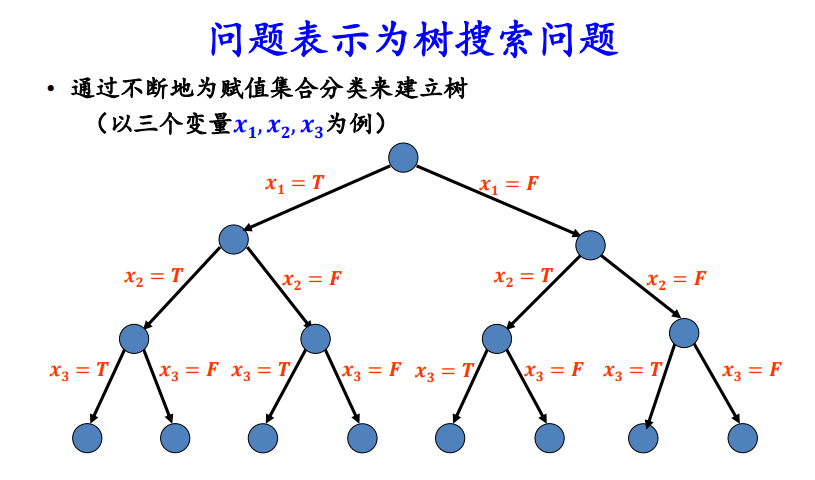
\includegraphics[scale = 0.5]{ss0.png}
        \caption{tu1}
    \end{figure}
\end{example}

\begin{example}[8-puzzle problem]
    就是那个, 不知道叫什么名字的那个. 见 Figure~\ref{tu2}. 我们这里进行的任何一个决策都能够表示为树. 
    你看, 这个空位在右上角, 那么我们若是以这个为初始状态, 
    那么我们有两种选择, 3 向右移动, 或者是 4 向上移动. 见 Figure~\ref{tu3}
    \begin{figure}
        \centering
        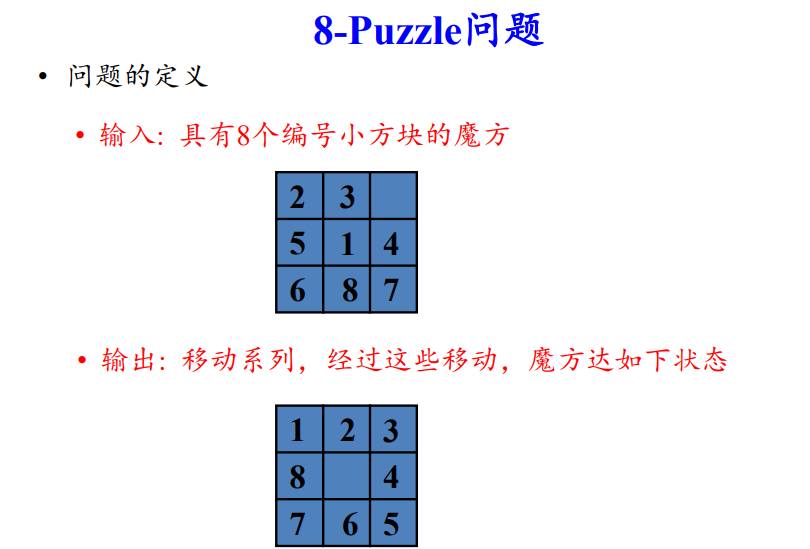
\includegraphics[scale = 0.5]{ss6.png}
        \caption{tu2}
        \label{tu2}
    \end{figure}
    \begin{figure}
        \centering
        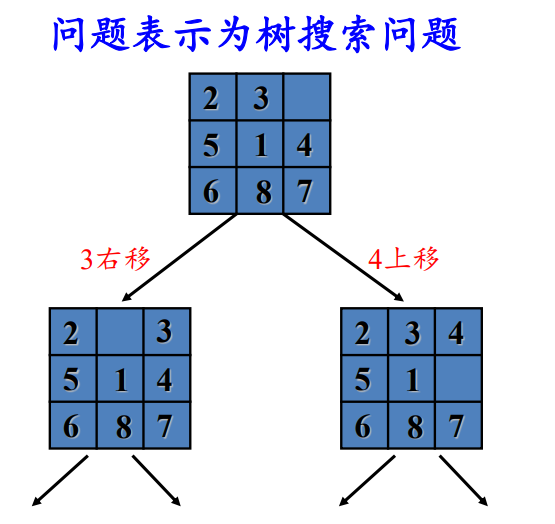
\includegraphics[scale = 0.5]{说是.png}
        \caption{tu3}
        \label{tu3}
    \end{figure}
\end{example}

\begin{example}[Hamiltonian 环问题]
让我们先定义一下, 我们有一个 $n$ 节点的连通图 $G = \left( V ,E\right)$. 我们需要知道, $G$ 中是否有
Hamiltonian 环. 

类似的, 我们知道, 每一个决策都能表示, 那么我们还可以表示环路. 
比如说我们从某一点出发, 那么`下一个点'有很多选择, 
那些没有经过的、相邻的点就行.
见Figure~\ref{tu4}
\begin{figure}
    \centering
    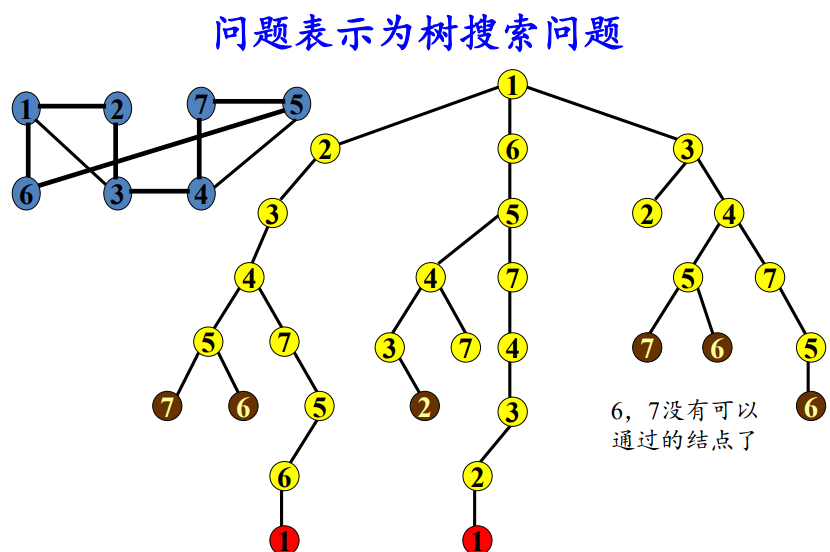
\includegraphics[scale = 0.5]{ss7.png}
    \caption{tu4}
    \label{tu4}
\end{figure}
\end{example}
\section{广度优先搜索和深度优先搜索}
我们以前接触过这两位, 是在学习树的时候.

与其说是两种策略, 不如说是使用了两种数据结构. 
深度优先是栈, 而广度优先是队列.

\subsection{BFS}
下面给出BFS的框架:

\begin{minted}[mathescape, 
                linenos, 
                numbersep=5pt,
                gobble=2,
                frame=lines,
                framesep=2mm]{c++}
    // 构造由根组成的队列 Q
    if Q 中的第一个元素 x 是目标节点
        stop
    else 
        从 Q 中删除 x, 将 x 的所有子节点放进 Q 中.
    if Q == NULL 
        return failed;
    else goto 2
\end{minted}
虽然使用了 \verb|goto| 但也算是简洁了, 其实用 \verb|while| 也很简洁. 
我们说这里的关键就是队列, 其特点就是先进先出. 
对于节点 $x$ , 我们将其子节点放入队列, 这些子节点都搞定之后才会继续搞其他的子节点.

\subsection{DFS}
区别在于使用了栈.

就是说, 我们一直走一直走, 然后走到终点, 才往回退, 
看看另一个选择, 总之就是先一条路走到黑. 使用栈的观点, 
会看的更清晰. 每次访问一个节点, 就将其子节点塞到栈里, 
然后取出站内的一个节点, 访问这个节点, 进行类似的操作. 
和广度优先遍历是完全类似的. 是不是非常神奇.
\begin{minted}[mathescape, 
                linenos, 
                numbersep=5pt,
                gobble=2,
                frame=lines,
                framesep=2mm]{c++}
    // 构造由根组成的栈 S
    if S 中的第一个元素 x 是目标节点
        stop
    else 
        Pop (S) ; 
        Push (s); // 将 S 的子节点压进栈.
    if S == NULL 
        return failed;
    else goto 2
\end{minted}
\section{搜索的优化}
\subsection{爬山法}
基本思想: 
在DFS的过程中, 使用贪心法确定搜索的方向. 
爬山策略使用 ``启发式函数'' 来排序节点优先程度. 

我们通过 $f$ 来测量某一个节点, 我们说, 
越接近某一值 $a$ 则该节点距离正确答案就越近, 
可以按照这一标准来排序节点. 

将当前节点 $x$ 的子节点压进栈的时候, 
按照上面的 ``启发式函数'' 给出的排列顺序压进栈.
实际上是一种贪心算法的思路. 

\begin{example}
    在 eight-puzzle 问题之中, 我们使用爬山法. 
    
    我们如下定义 ``启发式函数'' $f: V \to \mathbb{R}$, 其中, 我说, $V$ 是一个决策树上的节点的集合.
    并且 $f \left(n \right) $ 是当前情况之下, 处于正常位置的格子的个数. 见 Figure~\ref{tu5}.
    \begin{figure}
        \centering
        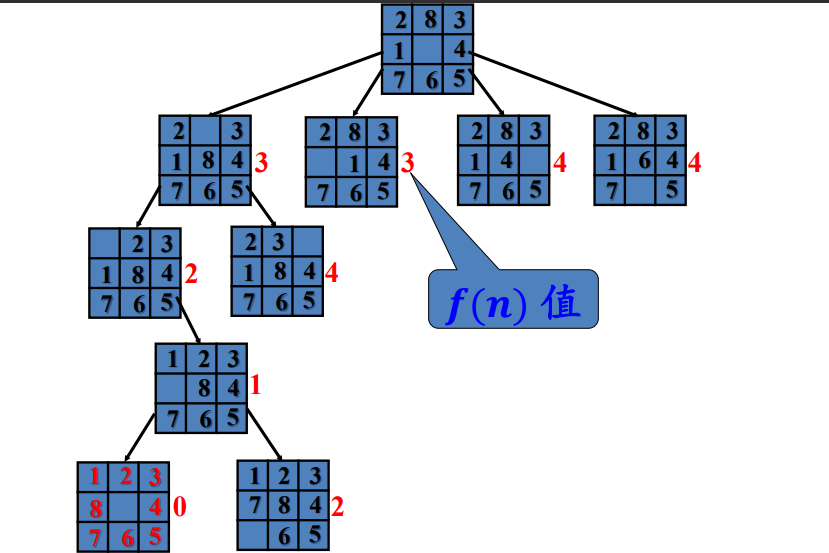
\includegraphics[scale = 0.5]{ss8.png}
        \caption{climb mountain in 8-puzzle}
        \label{tu5}
    \end{figure}
\end{example}

于是乎, 我们的算法思路就是这样:
\begin{minted}[mathescape, 
                linenos, 
                numbersep=5pt,
                gobble=2,
                frame=lines,
                framesep=2mm]{c++}
    // 构造由根组成的栈 S
    if S 中的第一个元素 x 是目标节点
        stop
    else 
        Pop (S) ; 
        Push (s); // 将 x 的子节点按照给出的排列顺序压入栈.
    if S == NULL 
        return failed;
    else goto 2
\end{minted}

我们能够明显地看出, 这个搜索策略并不一定是最优的策略\footnote{最优的策略应该很难找到吧}, 因为这只是一个贪心选择, 我们的问题不一定满足贪心选择性. 

接下来我们要修改的话, 就是考虑到全局的节点.
\subsection{Best-First 搜索}

类似的, 我们有给出一个函数 $f$ 来考察节点的优先程度.

基本思想: 将上面的这些数据结构换为 heap.
\begin{itemize}
    \item 结合深度优先和广度优先的优点
    \item 根据函数 $f$ 在目前产生的所有节点中选择具有最优的节点进行扩展 \footnote{扩展又是什么意思? 我不是说故意挑刺, 但是你不能总是突然冒出一个自己编篡的词语, 然后又不解释是什么意思}
    \item 选择了全局最优解, 而爬山只是局部最优.
\end{itemize}
\begin{minted}[mathescape, 
                linenos, 
                numbersep=5pt,
                gobble=2,
                frame=lines,
                framesep=2mm]{c++}
    依照 f 的值为比较的key, 构造出一个堆, 先是构造只有起点 r 的堆
    if H 的根 x 是目标节点 then stop;
    delete_max(H);  将 x 的子节点插入heap;
    if H == NULL then failed;
    else goto 2
\end{minted}
\subsection{分支界限}
基本思想: 
\begin{itemize}
    \item 上述方法很难用于求解优化问题 \footnote{为什么}
    \item 分支界限策略可以有效地求解组合优化问题. 
    \item 发现优化解的一个界限\footnote{就是硬求一个}, 缩小解空间, 提高求解的效率 \footnote{你在说什么}
\end{itemize}
\begin{example}
\begin{figure}[H]
    \centering
    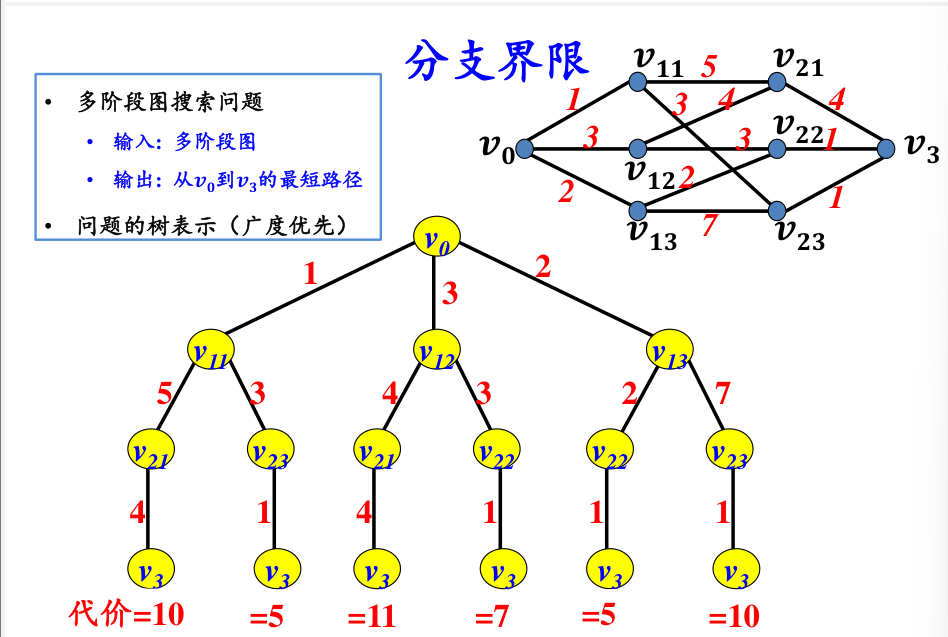
\includegraphics[scale=0.5]{ss1.png}
    \caption{例子}
    \label{tu6}
\end{figure}
\begin{itemize} 
    \item[1.] 图见 Figure~\ref{tu6}. 使用爬山策略, 找出一个路径(选择权重最小的边), 1 3 1 这条路
    \item[2.] 根据这个解, 进行剪枝. 已知这个路径的长度是 5 , 我们将上一层节点中大于 5 的节点剪去. 这就是缩小了解的范围.  
\end{itemize}
\end{example}
应该是剪完了之后遍历吧, 挺无语的. 总之分支界限的方法是:
\begin{enumerate}
    \item 产生分支的机制
    \item 产生一个界限
    \item 进行一个分支界限搜索, 
    剪除那些不可能产生
    优化解的分支.
\end{enumerate}
\section{剪枝方法与人员安排问题}
\subsection{问题初步处理}
\subsubsection{问题描述}
\noindent $\mathbf{input}:$ 人员安排的问题之定义实际上是这样, 我们有一个工作的集合:
\begin{definition}
$J = \left\{J_{i}\right\}_{i \in \mathbb{N}}$, 
他是一个偏序集, 我们将其进行一个拓扑排序
\footnote{什么是拓扑排序来着}
\end{definition}
比如说我们有一个排序, $\left\{J_{i_{k}}\right\}$ $J_{i_{k}}$ 是排序中的第 $k$ 个工作,
意思就是这个工作由第 $k$ 个人来担任.
\begin{definition}
同时给出了一个矩阵 $C = \left(c_{ij}\right)$ , 
$c_{ij}$ 的意思是, 第 $i$ 个
人分配了第 $j$ 个工作所需要的时间. 
\end{definition}
\begin{corollary}
    符号写得非常差劲捏.
\end{corollary}

\noindent \textbf{output:}矩阵 $X = \left(x_{ij}\right) , x_{ij} \in \left\{ 0 , 1\right\}$ 
满足
\begin{align*}
    \sum_{i, j }  c_{ij} x_{ij} 
\end{align*}
viz. 工作所需要的代价最小.
\begin{figure}
\centering
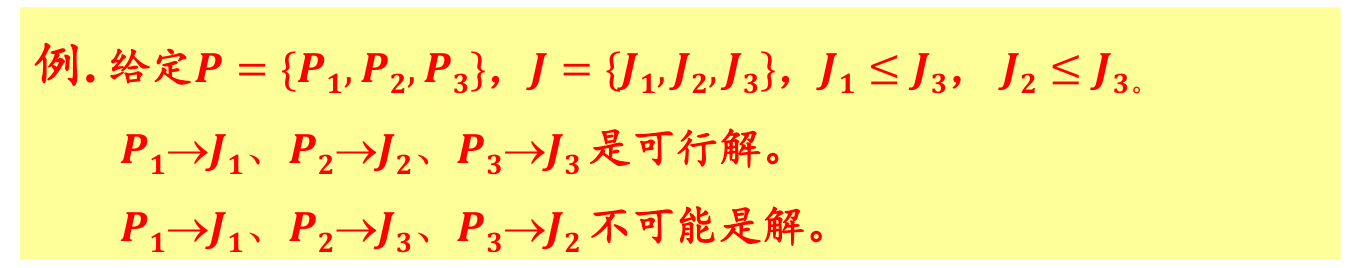
\includegraphics[scale = 0.4]{ss2.png}
\caption{一个例子}
\label{fig:tu7}
\end{figure}
我们这里有一个拓扑排序的例子, 见 Figure~\ref{fig:tu7}
\subsubsection{求解思路}
于是说, 我们的目的就是要遍历所有的拓扑排序, 
从中找到一个最优解, 总体来说这是一个遍历的过
程. 我们可以回想以前是怎么找拓扑排
序的: 每次选择一个 ``没有前序元素的'' 的
元素, 作为当前根节点的子节点. 
对于这些获得的子节点也是使用这样方法, 也就是递归地处理子节点. 
能够看出这其中的这个决策就是 ``选取这些没有前序元素的元素'', 于是
我们能够画出这个决策树, 将每一个topo排序列出来, 
进行一个搜索.

\subsubsection{topo排序}
\begin{enumerate}
    \item 
生成空树根 
\item
选择偏序集中没有前序元素的元素, 作为当前根节点的子节点
\item
For root 的每一个子节点, do 
\item
$S = S  - \left\{v\right\}$
\item 
将 $v$ 作为根, 递归地处理 $S$
\end{enumerate}
我们这就生成了一个拓扑排序对应的树, 这个树上, 从根
节点到叶子的一条路就是一个拓扑排序.

我们接下来的目的是对这个方法进行一个优化.

\subsection{算法的优化: 针对代价矩阵做出的优化}
\begin{proposition}
    将代价矩阵的一行或者一列, 减去同一个数字, 不影响优化解的求解.\footnote{这该怎么证明?}
\end{proposition}
\begin{itemize}
    \item 代价矩阵的每行减去同一个数, 使得每一行
    以及每一列是找有一个零, 其余元素非负. 
    \item 减数的和是解的一个下界. 
\end{itemize}    
显然, 这个下界没什么用, 不能剪枝啊. 能有什么用? 但是这并不能直接
忽略了, 我们将其放在根节点上, 这样靠谱吧. 

\begin{example}
我们有一个代价矩阵:
\[
\begin{bmatrix}
    29 & 19 & 17 & 12 \\
    32 & 30 & 26 & 28 \\
    3 & 21 & 7 & 9\\
    18 & 13 & 10 & 15
\end{bmatrix}
\]
第一行 $-12$ , 第二行 $-26$ , 第三行 $-3$ , 第四行 $-10$, 有 
\[
\begin{bmatrix}
    17 &  7 & 5 & 0 \\ 
    6 & 4 & 0 & 2 \\
    0 & 18 & 4 & 6 \\
    8 & 3 & 0 & 5
\end{bmatrix}
\]
第二行能够 $-3$, 于是就有 
\[
\begin{bmatrix}
    17 & 4 & 5 &  0 \\ 
    6 & 1 & 0 & 2 \\
    0 & 15 & 4 & 6\\
    8 & 0 & 0 & 5
\end{bmatrix}
\]
\begin{figure}
    \centering
    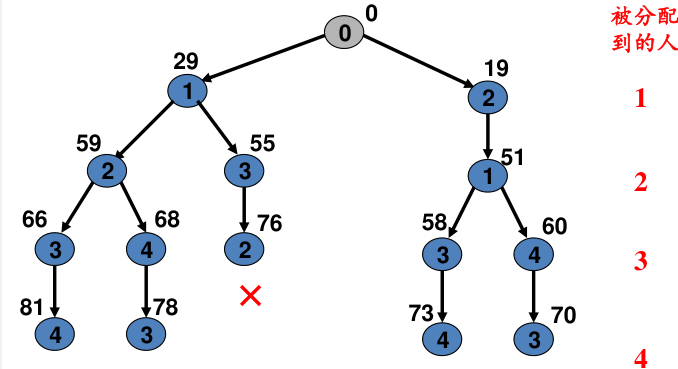
\includegraphics[scale = 0.5]{ss3.png}
    \caption{优化前的树}
    \label{fig:tu8}
\end{figure}
\begin{figure}
    \centering
    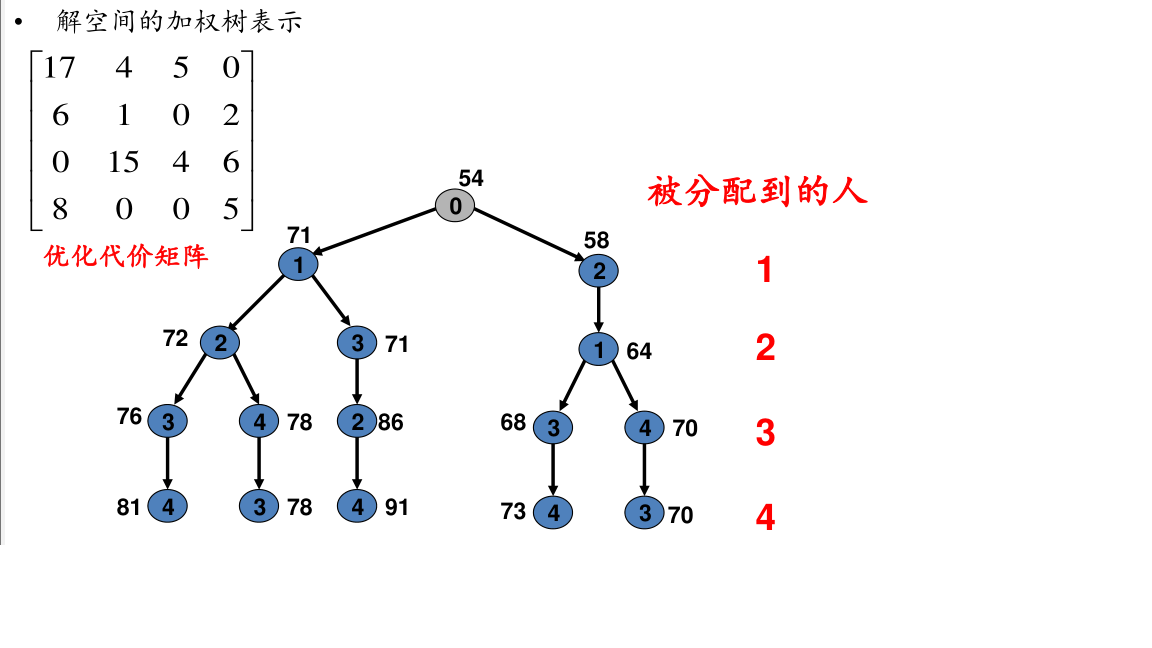
\includegraphics[scale =0.5]{ss4.png}
    \caption{优化后的树}
    \label{fig:tu9}
\end{figure}

我们根据两个矩阵还有那个偏序集, 画出决策树. 见 Figure~\ref{fig:tu8} 以及 Figure~\ref{fig:tu9}.
能够看出, 进行优化之前的树剪了个寂寞, 就剪了一个, 没啥用. 但是优化之后就比较猛了. 
我们选到的是 $70$ 作为一个解的上界, 左边那个子树能够剪掉很多分支. 见 Figure~\ref{fig:tu10}
\begin{figure}
    \centering
    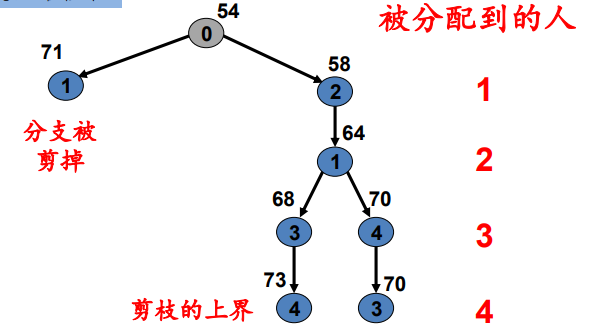
\includegraphics[scale = 0.5]{ss9.png}
    \caption{优化后剪枝}
    \label{fig:tu10}
\end{figure}
\end{example}
\section{旅行商问题}
\subsection{问题描述}
在一个有向图中, 找到一个路径最短的 Hamiltonian 回路.
\subsection{求解思路} % (fold)
\label{sub:silu}
这个玩意的求解思路有一些复杂, 
我们现在阐述一下.
我们仍然使用决策树, 根节点放着的是所有可行解的集合.
使用爬山方划分空间, 
得到一个二叉树. 按照ppt上的说法是这样的, 并且划分方法是
如下:
\begin{enumerate}
    \item 选定一个边 $\left(u  ,v\right)$
    \item 包含了 $\left( u ,v\right) $ 的解作为左子树, 
    不包含 $\left( u ,v\right)$ 的解, 作为右边子树.
    \item 我们根据这种信息, 更新左右两边的代价下界. 
    \item $\left( u ,v\right)$ 的选择原则是, 优化后的代价矩阵中 $ \left( u ,v\right)$ 
    的值等于 $0$ , 并且, 右子树代价下界直接增加值\footnote{什么是直接增加值}最大.
\end{enumerate}
% subsection test (end)
\subsection{如何更新左子树的下界} % (fold)
\label{sub:如何更新左子树的下界}
简单来说, 就是使用了这个 $\left( u ,v\right) $ 那么, 有一些边就可以直接不选了, viz. 
以 $u$ 为起点, 以及以 $v$ 为终点那些边都不选了. Moreover, $\left( v, u\right)$ 也不能选了.

我们画个图就明白了, 比如说我们选取了 $\left( 4 , 6\right)$
\[
\begin{bmatrix}
    \infty & 0 & 83 & 9 & 30 & 6 & 50 \\
    0 & \infty & 66 & 37 & 17 & 12 & 26 \\
    29 & 1 & \infty & 19 & 0 & 12 & 5\\
    32 & 83 & 66 & \infty & 49 & 0 & 80 \\
    3 & 21 & 56 &  7 & \infty &  0& 28\\
    0 & 85 & 8 & 42 & 89 & \infty & 0\\
    18 & 0 & 0 & 0 & 58 & 13 & \infty 
\end{bmatrix}\rightarrow
\begin{bmatrix}
    \infty & 0 & 83 & 9 & 30 & \text{foo}  & 50 \\
    0 & \infty & 66 & 37 & 17 &\text{foo} & 26 \\
    29 & 1 & \infty & 19 & 0 &\text{foo}& 5\\
    \text{foo} & \text{foo} & \text{foo} & \text{foo} &\text{foo} &\text{foo}  &\text{foo} \\
    3 & 21 & 56 &  7 & \infty &  \text{foo}& 28\\
    0 & 85 & 8 & \text{foo} & 89 &\text{foo}& 0\\
    18 & 0 & 0 & 0 & 58 &\text{foo}& \infty 
\end{bmatrix}
\]
这个时候, 我们还可以进行矩阵的优化, 就是说在某一些行里面减去一些东西, 使得其代价的下界增加了. 比如说这里就是三
% subsection 如何更新左子树的下界 (end)
\subsection{如何更新右子树的下界} % (fold)
\label{sub:如何更新右子树的下界}
我们说, 如果说我们不再选择这个 $ \left( u , v\right)$ 那么一定会有一个边是以 $u$ 为起点, 而另一个边是 $v$ 为终点的.
注意这里的措辞, 这里是两个边, 你想想, 对于每一个点, 实际上都有一进一出的边, 
这里的重点在于, 现在是两个边或者以上, 用来连接 $\left( u , v\right)$. 

与上面的有些相反, 我们要找到 $u$ 为起点的最短的那个边, 以 $v$ 为终点的那个边. 
\[
\begin{bmatrix}
    \infty & 0 & 83 & 9 & 30 & 6 & 50 \\
    0 & \infty & 66 & 37 & 17 & 12 & 26 \\
    29 & 1 & \infty & 19 & 0 & 12 & 5\\
    32 & 83 & 66 & \infty & 49 & 0 & 80 \\
    3 & 21 & 56 &  7 & \infty &  0& 28\\
    0 & 85 & 8 & 42 & 89 & \infty & 0\\
    18 & 0 & 0 & 0 & 58 & 13 & \infty 
\end{bmatrix}
\]
以这个为例子, 能够找到第四行中, 最小的是 32. 第 6 列中, 最小的是 0.
那么这个代价下界就增加了 $32 + 0 = 32$ 
这样的增加就是直接增加.

并且我们说, 还有另一种表述方法, 不能使用 $\left(  u ,v\right)$ 其实相当于这个边的权重变为 $ \infty  $ .
% subsection如何更新右子树的下界 (end)
\subsection{实例} % (fold)
\label{sub:实例}
下面是一个实例. L.B. 的意思是 Lower Bound
\begin{figure}
    \centering
    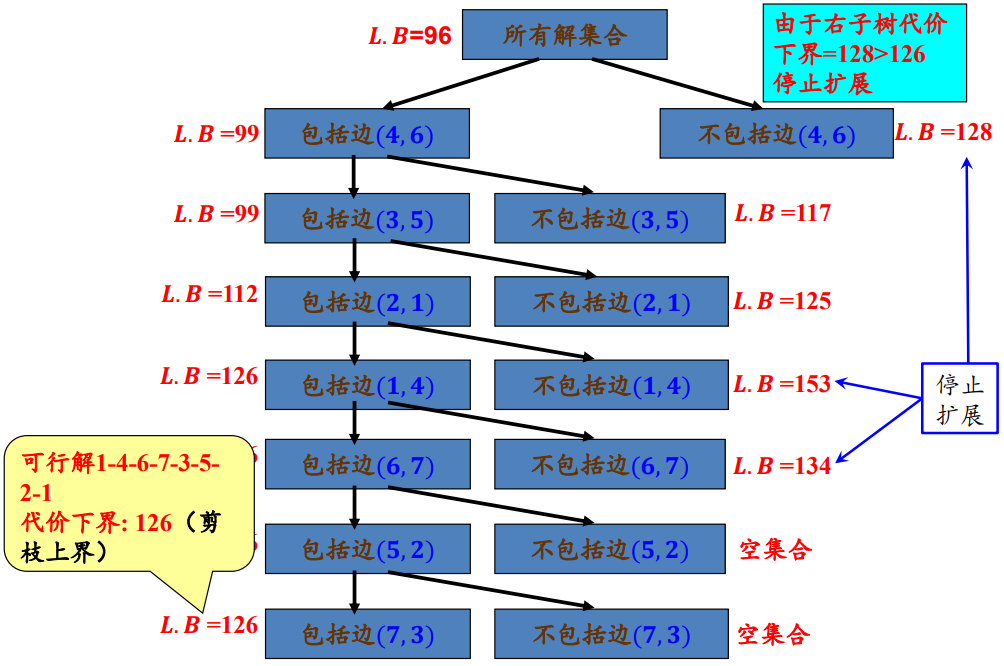
\includegraphics[scale = 0.5]{ss10.png}
    \caption{实例}
    \label{fig:tu11}
\end{figure}
% subsection实例 (end)

\section{A*算法}
\subsection{代价函数$f*$} % (fold)
\label{sub:代价函数}
在这里, 我们以图最短路径为例, 
我们说 $g\left(n\right)$ 是 $n$ 节点
到目标节点的优化路径的代价. 
$f^{*}\left( n\right) = g\left(n\right) + h ^{*} \left(n\right)$ 是节点 $n$ 的代价.

但是我们不知道, $h ^{*} \left(n\right)$ 的值, 因为我们不知道 $h ^{*} \left( n\right)$ 的值. 
我们还是能够使用某些方法进行这个 $h ^{*} \left(n\right)$ 的估计. 
比如说, 一个点, 他不是终点, 那么他到终点, 至少还有要走一个边, 
那么, $h ^{*} \left(n\right)$ 的值一定大于, 
这个相邻的边之中最小的那个. 
这就是 $h ^{*} $ 的一个估计.

说实话非常粗糙.

% subsection 代价函数 (end)
\subsection{图解过程} % (fold)
\label{sub:图解过程}

我们说, 这个 $A ^{*}$ 算法其实不是很难, 但是我们要熟悉这个概念, 并且熟悉这个操作. Figure~\ref{fig:tujie} 
是一个实例. 我们只需要记住, 这个步骤其实非常简单, 就是best-first 
方法加上那个什么 $f ^{*} $ 函数, 
一点点小优化而已.
\begin{figure}
    \centering
    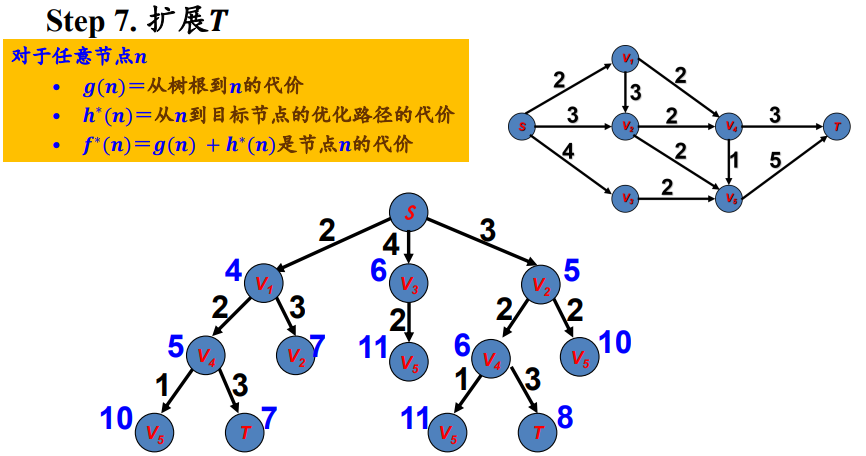
\includegraphics[scale = 0.5]{ss11.png}
    \caption{图解}
    \label{fig:tujie}
\end{figure}
% subsection图解过程 (end)
\subsection{算法正确性证明} % (fold)
\label{sub:算法正确性证明}
\begin{theorem}
使用 Best-first 策略搜索树, 
如果说 $A ^{*}$ 选择的是目标节点, 
那么该节点表示的解是优化解.
\end{theorem}

\begin{proof}
设 $T$ 是目标节点, $T$ for target. 我们需要证明 $f\left(T\right)$ 是最优的.
\begin{enumerate}
    \item A$^{*}$ 使用的是 Best-first, 那么说 对于当前任意的, 还没有被扩展的节点 $v$
    来说, $f\left(T\right) \le f \left(v\right)$
    \item 因为对于任意的顶点 $v$ 来说, $f \left( v\right) \le f ^{*} \left(v\right)$ ,
所以说, $\forall  v \in V, f \left(T \right) \le f ^{*} \left(v\right)$
    \item $\left\{ f^*\left(v\right)\right\}_{v \in V}$ 中一定有一个是最优的\footnote{are you sure}, 设
    其为 $s$ , 对应的代价为 $f ^{*} \left(s\right)$ 
    \item 明显 $g \left(T\right) =  f\left(T\right)$, 这是因为 $h \left(T\right)   = 0 $  
    所以说 
    \begin{align*}
        g\left(T\right)  \le f ^{*} \left(s\right)
    \end{align*}
    \item 因为 $f ^{*} \left(s\right) $ 是最优的, 那么说, 所有到 $T$ 的路径长度都小于 $f^{*} \left(s\right)$, i.e. $g\left(T\right) \ge f^{*} \left(s\right)$
    综合一下就有 
    \begin{align*}
        g\left(T\right) = f ^{*} \left(s \right) \quad \quad \qedhere
    \end{align*} 
\end{enumerate}
\end{proof}

\begin{proof}[另一个证明]
    设A*算法找到了路径 $P$, 这个路径来到了终点 $T$ , 然后我说, 这个路径实际上不是最小的. 
    
    然后说, 有另一个更小的路径 $Q$ . 既然说这两个路径是不一样的, 
    那么说 $Q$ 一定存在节点 $v$
    不在路径 $P$ 之中 (are you sure)
    
    设从 $v$ 开始, 两个路径开始不同, 有:
    \begin{align*}
        f\left(v\right) \le g_{Q}\left(T\right)  < g_{P}\left(T\right) \le f\left(T\right)
    \end{align*}
    于是就有, $f \left(v\right) \le f \left(T\right)$. 这和什么矛盾呢? 
    这就和 Best-first 方法矛盾了.
\end{proof}
% subsection 算法正确性证明 (end)
\end{document}